\chapter{Methodology}
\label{ch:methodology}

\section{Overview of the Approach}

This project employs a dual-approach methodology for extracting causal relationships from World War I historical documents. The two approaches are:

\begin{enumerate}
    \item \textbf{Rule-Based Approach:} Uses linguistic patterns, semantic similarity, and entity matching to identify causal relationships
    \item \textbf{Hybrid Machine Learning Approach:} Combines rule-based filtering with transformer-based Natural Language Inference for enhanced accuracy
\end{enumerate}

Both approaches share a common preprocessing pipeline and validation framework, but differ in their core extraction mechanisms. This chapter details the theoretical foundations and algorithmic design of each approach.

\section{System Architecture}

The overall system architecture consists of three main modules:

\begin{figure}[H]
    \centering
    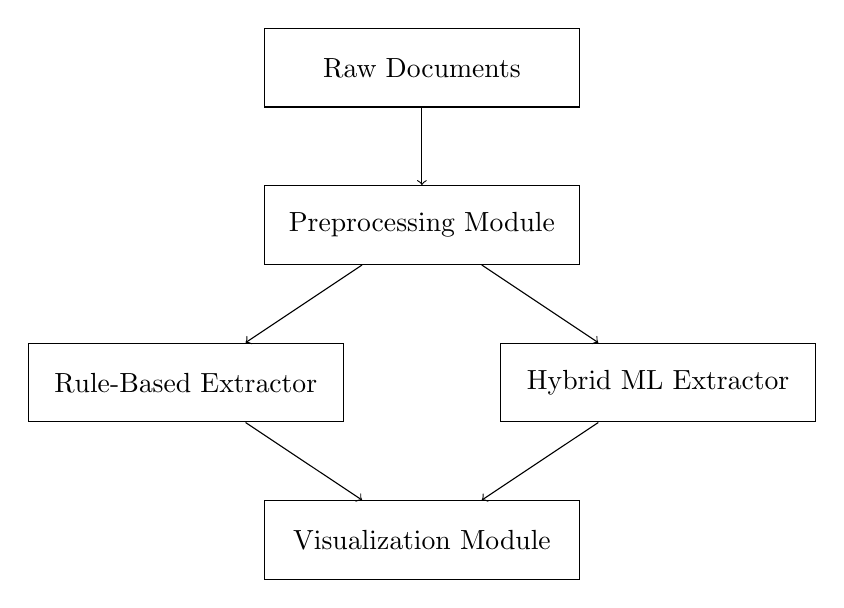
\begin{tikzpicture}[node distance=2cm, auto]
        \node[draw, rectangle, minimum width=4cm, minimum height=1cm] (input) {Raw Documents};
        \node[draw, rectangle, minimum width=4cm, minimum height=1cm, below of=input] (preprocess) {Preprocessing Module};
        \node[draw, rectangle, minimum width=4cm, minimum height=1cm, below of=preprocess, xshift=-3cm] (rulebased) {Rule-Based Extractor};
        \node[draw, rectangle, minimum width=4cm, minimum height=1cm, below of=preprocess, xshift=3cm] (ml) {Hybrid ML Extractor};
        \node[draw, rectangle, minimum width=4cm, minimum height=1cm, below of=rulebased, xshift=3cm] (viz) {Visualization Module};
        
        \draw[->] (input) -- (preprocess);
        \draw[->] (preprocess) -- (rulebased);
        \draw[->] (preprocess) -- (ml);
        \draw[->] (rulebased) -- (viz);
        \draw[->] (ml) -- (viz);
    \end{tikzpicture}
    \caption{High-Level System Architecture}
    \label{fig:architecture}
\end{figure}

\section{Data Preprocessing}

\subsection{Document Collection}

The dataset comprises 1,490 historical documents related to World War I. The documents are categorized into several types:

\begin{table}[H]
    \centering
    \caption{Document Categories in the Dataset}
    \label{tab:doc-categories}
    \begin{tabular}{lcc}
        \toprule
        \textbf{Category} & \textbf{Count} & \textbf{Description} \\
        \midrule
        Personal Letters & 680 & Letters between soldiers and families \\
        Diary Entries & 450 & Personal diary records from soldiers \\
        Battle Accounts & 120 & Descriptions of military engagements \\
        Historical Records & 85 & Official and academic historical texts \\
        Survivor Accounts & 155 & Oral history transcripts \\
        \bottomrule
    \end{tabular}
\end{table}

\subsection{Text Normalization}

The preprocessing pipeline applies the following normalization steps:

\begin{enumerate}
    \item \textbf{Character Encoding:} Convert all documents to UTF-8 encoding
    \item \textbf{Sentence Segmentation:} Split documents into individual sentences using punctuation-based heuristics
    \item \textbf{Text Cleaning:} Remove or normalize special characters, excessive whitespace, and formatting artifacts
    \item \textbf{Tokenization:} Split text into individual tokens (words) for analysis
\end{enumerate}

\subsection{Sentence Filtering}

Not all sentences in the documents are suitable for causal extraction. The system applies filters to identify candidate sentences:

\begin{itemize}
    \item Minimum length threshold (50 characters) to ensure sufficient context
    \item Detection of causal language markers
    \item Presence of action or consequence indicators
\end{itemize}

\section{Rule-Based Extraction Methodology}

\subsection{Causal Language Detection}

The rule-based approach identifies causal relationships through linguistic patterns. Two categories of patterns are used:

\subsubsection{Forward Causal Patterns}

These patterns indicate that the cause precedes the effect in the sentence structure:

\begin{itemize}
    \item \texttt{caused | led to | resulted in | triggered | sparked | brought about}
    \item \texttt{consequently | therefore | thus | hence | as a result}
    \item \texttt{in response to | following | after the | due to the}
    \item Conditional structures: \texttt{when ... then}
    \item Explanatory patterns: \texttt{because of the | because this}
\end{itemize}

\subsubsection{Reverse Causal Patterns}

These patterns indicate that the effect precedes the cause in the sentence structure:

\begin{itemize}
    \item \texttt{because | due to | owing to | on account of}
    \item \texttt{as a result of | in consequence of}
    \item \texttt{was caused by | resulted from}
\end{itemize}

\subsection{Entity Extraction}

The system identifies named entities relevant to WWI historical context:

\begin{itemize}
    \item \textbf{Battle Names:} Somme, Verdun, Ypres, Passchendaele, Marne, Gallipoli, etc.
    \item \textbf{Geographic Locations:} France, Belgium, Flanders, Egypt, Palestine, etc.
    \item \textbf{Military Units:} Battalion, Brigade, Division, Regiment, Corps
    \item \textbf{Nationalities:} Australian, British, French, German, Turkish
    \item \textbf{Temporal References:} Dates in format ``Month Year'' or standalone years
    \item \textbf{Proper Nouns:} Capitalized words not in exclusion list
\end{itemize}

\subsection{TF-IDF Based Semantic Similarity}

To measure the semantic relatedness of potential cause-effect pairs, the system employs TF-IDF (Term Frequency-Inverse Document Frequency) vectorization with cosine similarity.

\subsubsection{IDF Computation}

For each word $w$ in the vocabulary, the IDF score is calculated as:

\begin{equation}
    IDF(w) = \log\left(\frac{N}{1 + df(w)}\right)
\end{equation}

where $N$ is the total number of documents and $df(w)$ is the document frequency of word $w$.

\subsubsection{TF-IDF Vectorization}

For a given sentence, the TF-IDF weight for word $w$ is:

\begin{equation}
    TFIDF(w) = TF(w) \times IDF(w) = \frac{f(w)}{max\_freq} \times IDF(w)
\end{equation}

where $f(w)$ is the frequency of word $w$ in the sentence and $max\_freq$ is the maximum frequency of any word in the sentence.

\subsubsection{Cosine Similarity}

The similarity between two sentences is computed as:

\begin{equation}
    sim(S_1, S_2) = \frac{\sum_{w \in S_1 \cap S_2} TFIDF_1(w) \times TFIDF_2(w)}{\sqrt{\sum_{w \in S_1} TFIDF_1(w)^2} \times \sqrt{\sum_{w \in S_2} TFIDF_2(w)^2}}
\end{equation}

The similarity score is used to filter pairs:
\begin{itemize}
    \item Minimum threshold (0.15): Ensures some semantic overlap
    \item Maximum threshold (0.65): Prevents near-duplicate sentences
\end{itemize}

\subsection{Confidence Scoring}

The rule-based system assigns confidence scores based on multiple criteria:

\begin{table}[H]
    \centering
    \caption{Confidence Score Components}
    \label{tab:confidence-scores}
    \begin{tabular}{lc}
        \toprule
        \textbf{Criterion} & \textbf{Score Contribution} \\
        \midrule
        Causal phrase in cause sentence & +0.30 \\
        Causal phrase in effect sentence & +0.25 \\
        High semantic similarity (0.25-0.50) & +0.20 \\
        Moderate semantic similarity (0.15-0.25) & +0.10 \\
        Shared entities (up to 3) & +0.08 per entity \\
        Action indicators in cause & +0.10 \\
        Consequence indicators in effect & +0.10 \\
        \bottomrule
    \end{tabular}
\end{table}

The minimum confidence threshold for acceptance is 0.85.

\section{Hybrid Machine Learning Methodology}

\subsection{Architecture Overview}

The hybrid approach combines rule-based filtering with ML-based validation:

\begin{enumerate}
    \item Apply rule-based filtering to identify candidate pairs
    \item Use NLI model to score causal plausibility
    \item Combine rule and ML scores for final ranking
\end{enumerate}

\subsection{Natural Language Inference Model}

The system uses the DistilBART-MNLI model from Hugging Face:

\begin{itemize}
    \item \textbf{Model:} \texttt{valhalla/distilbart-mnli-12-3}
    \item \textbf{Architecture:} Distilled BART with 12 layers
    \item \textbf{Training Data:} Multi-Genre Natural Language Inference corpus
    \item \textbf{Task:} Zero-shot classification
\end{itemize}

\subsection{Causal Validation via Entailment}

The NLI model evaluates whether a cause-effect relationship is plausible by testing entailment. The input is formatted as:

\begin{quote}
    ``[Cause text]. As a result, [Effect text]''
\end{quote}

The model classifies this combined text against two labels:
\begin{itemize}
    \item ``causal relationship''
    \item ``unrelated''
\end{itemize}

The probability assigned to ``causal relationship'' becomes the ML score.

\subsection{Combined Scoring}

The final score for each pair combines rule-based and ML scores:

\begin{equation}
    score_{combined} = \frac{score_{rule} + score_{ML}}{2}
\end{equation}

This averaging approach balances linguistic pattern evidence with semantic plausibility assessment.

\section{Validation Criteria}

Both approaches enforce strict validation criteria:

\begin{enumerate}
    \item \textbf{Cross-File Requirement:} Cause and effect must come from different source documents
    \item \textbf{Minimum Length:} Both sentences must exceed 50 characters
    \item \textbf{Causal Language:} At least one sentence must contain causal markers
    \item \textbf{Semantic Similarity:} Similarity score between 0.15 and 0.65
    \item \textbf{Shared Context:} At least 2 shared entities between sentences
    \item \textbf{Confidence Threshold:} Final score must meet minimum threshold
\end{enumerate}

\section{Network Visualization}

Extracted relationships are represented as directed graphs:

\begin{itemize}
    \item \textbf{Nodes:} Represent cause or effect events
    \item \textbf{Edges:} Directed edges from cause to effect
    \item \textbf{Edge Weights:} Confidence scores
    \item \textbf{Node Colors:} Distinguish cause nodes (blue) from effect nodes (green)
\end{itemize}

The NetworkX library is used for graph construction, and matplotlib generates the visualizations.

\section{Summary}

This chapter has presented the methodological framework for causal relationship extraction. The rule-based approach relies on linguistic patterns and semantic similarity, while the hybrid approach adds machine learning validation. Both approaches share preprocessing and validation components, ensuring consistency in the extraction pipeline. The following chapter details the technical implementation of these methods.
